\setstretch{1.6}
\sectiontitle{6}{Closed-Loop Tension Control}
\lhead{Closed-Loop Tension Control} % section header
As mentioned in the project context a form of closed-loop control of the tendon tensions was already implemented before the start of this thesis. However that implementation had several issues, including large steady state error up to 100mN, and difficulty in tracking the setpoints when while the linear stage was moving, thereby creating large over- and undershoots in tension. There were also issues in the implementations of the GUI leading the setpoint to be set to zero before being set to the desired setpoint decided by the user. Therefore it was necessary to rework this closed-loop tension control in order to ensure that later navigational control that would be implemented on top of this inner closed loop would function in the intended manner.

\lhead{Closed-Loop Tension Control - Methods} % section header
\subsection{Methods}

\subsubsection{System Analysis and Initial PID Tuning}
In order to rework the closed-loop tension control it was necessary to first figure out what was leading to the poor functionality. To investigate this a logger was implemented that logged and saved all relevant data. A script for analyzing and plotting the data was also written in python. 
\newline \newline
After analyzing the behavior, the simplest solution was tested first, namely retuning the PIDs, especially turning up the integral term. However returning in an attempt to remove the standard deviation led to instability, oscillations and large errors particularly when the ribbon was being moved up and down by the linear stage. Therefore the entire PID implementation had to be re-evaluated and re-worked. 

\subsubsection{Identifying Control Limitations due to Hardware}
The observed instability and failure to reach tension setpoints was ultimately traced back to limitations due to utilizing a speed controller for the Faulhaber brushless motors used in the system. A speed controller is not well suited for tension control since it is designed to regulate the motor's rotational speed, not the force (torque) it applies to maintain tension. In tension control, the goal is to keep a consistent pulling force on the tendon, which depends directly on the motor's torque. However, a speed controller adjusts torque only as a means to achieve a target speed. Thus in this original implementation where a closed-loop PID tension control is implemented on top of a speed controller, the layered control structure causes significant issues. The outer tension control loop adjusts the target speed command based on the tension error, but it takes time for the inner speed controller to reach this set target, in the mean time the outerloop will continue to recalculate the speed setpoints. So if the outerloop sets a speed target that the inner loop can not reach before the outerloop calculates a new setpoint, there is in-effect a significant delay that leads to instability. 
\newline \newline
Because of these dynamics, an attempt was made to change the parameters of the speed controller by turning down the proportional term of the internal speed PID controller and setting the integral term to zero. The aim was to gain more direct control of the motor's behavior by reducing the internal controller's influence, allowing the outer tension loop to act more like a direct torque controller. However it turned out to be impossible to turn of the integral term, apparently the internal PID parameters, particularly the integral term, are auto-configured and to a degree locked by the Motion Manager software and not intended for external adjustment. Since it was impossible to turn of the integral term this led to undesired behavior, such as when the motor is given a constant setpoint it will begin by reeling in the string as intended, but then will slowly stop reeling in and eventually start turning the other way, releasing the string until it is manually stopped. 

\subsubsection{System Adaptation Strategy}
Since the inner controller could not be reconfigured for torque control, the solution was to adapt the system to work within these constraints. This means making the inner loop, i.e. the motor's internal speed control, as fast and responsive as possible. In contrast, everything else around the motor has to be slowed down to avoid overwhelming the inner loop.
\newline \newline
This also requires making the brush less motors as responsive as possible, so to that end the deadzone for the motors was found and compensated for in the implementation of the controller. Additionally it was important to ensure that the sensor were as accurate as possible, thus they were recalibrated and tare-ing functionality was implemented.

\subsubsection{Integration of New Hardware}
However before doing so the setup was due for another iteration. There were several issues with the initial implementation of the system including unreliable reeling in of the tendons, the backbone would also often slip leading to unreliable behavior. Therefore the mechanical setup redesigned by Lorenzo and the motor responsible for moving the backbone of the tendon up and down was replaced. It was therefore a necessary step to assemble the setup once the components arrived, redo the wiring and write a control class in C++ for the new linear stage and integrate it with the rest of the codebase. A comparison between the previous hardware iteration and the new hardware assembled during this thesis can be seen in figure \ref{fig:hardwarecompare}.
\newline \newline
The \texttt{LinearStageController} class was implemented by adapting C++ example code and API documentation provided by Physik Instrumente. Core functionality such as motion control, servo handling, and data recording was tailored to the system using these references. The code was modularized, integrated with Qt’s signal-slot system, and extended with safety checks and asynchronous timers to meet real-time control and estimation requirements.

\begin{figure}[H]
    \centering
    \begin{subcaptionbox}{Old Setup\label{fig:left}}[0.5\linewidth]
        {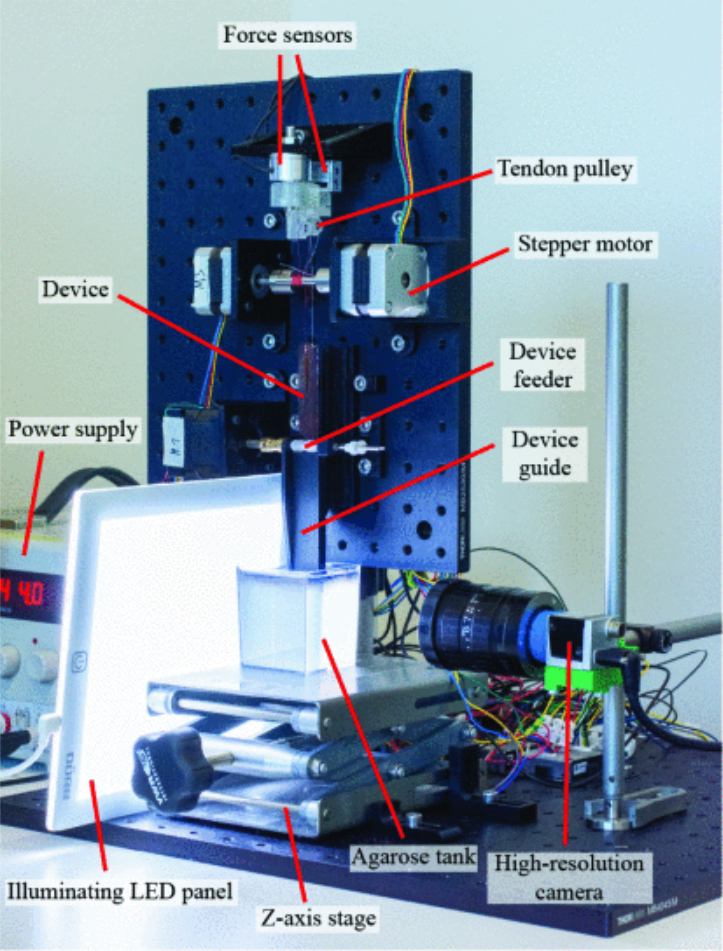
\includegraphics[width=\linewidth]{images/Hardware/old.PNG}}
    \end{subcaptionbox}
    \hspace{0.05\linewidth}
    \begin{subcaptionbox}{New Setup\label{fig:right}}[0.4\linewidth]
        {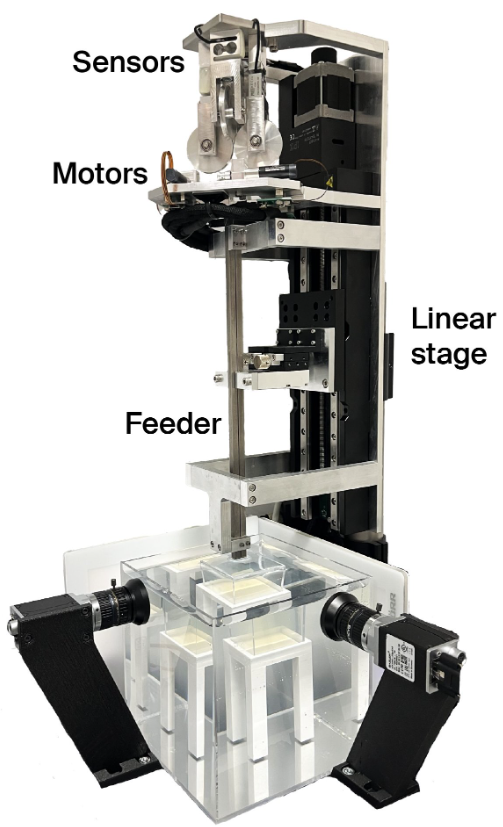
\includegraphics[width=\linewidth]{images/Hardware/insertionStrategy.PNG}}
    \end{subcaptionbox}
    \caption{Comparison of the previous hardware iteration (a) and the new hardware (b) assembled during this thesis}
    \label{fig:hardwarecompare}
\end{figure}


\subsubsection{Validation Strategy}
\todo{write section?}


\subsection{Design}

\todo{figure of the closed loop for tendon tension}


\lhead{Closed-Loop Tension Control - Implementation} % section header
\subsection{Implementation}
\todo{Write small section syaing this section details the implementation of the boxes in the closed loop tendon tension control}

\subsubsection{Brushless motor speed controller}
Since the inner controller is a speed controller and could not be recongifured for torque control, the solution was to instead optimize the system around its limitations. This involved selecting the best parameters for the inner speed controller to ensure that it responds as quickly as possible. This turned out to be the values provided by Faulhaber as default values. 

\subsubsection{Linear stage speed feedforward}
Since the backbone of the ribbon is moved up and down by the linear stage and the tendons are attached at the distal most point of the ribbon, it makes sense to have a feedforward to the tendon tension control that ensures that the tension remains relatively stable during movement by reeling the appropriate amount in or out based on the speed of the linear stage. This also ensures that the feedback doesn't need to do all the heavy lifting of compensating for the movement.

\paragraph*{Implementing a new linear stage}
Before moving on to implementing the feedforward element that depends on the speed of the linear stage, the new linear stage had to be implemented. In a previous iteration of the system, the one that was implemented when this thesis was started the setup utilized a servomotor along with with a "feeder" that consisted of two counterrotating barrels, essentially serving as a conveyor belt. However there were significant issues with this mostly due to slipping, something that was exacerbated when the system was miniaturized. It was therefore replaced by a linear stage that is directly attached to the top of the ribbon, removing the slipping issue of the conveyor belt solution.

\begin{figure}[H]
    \centering
    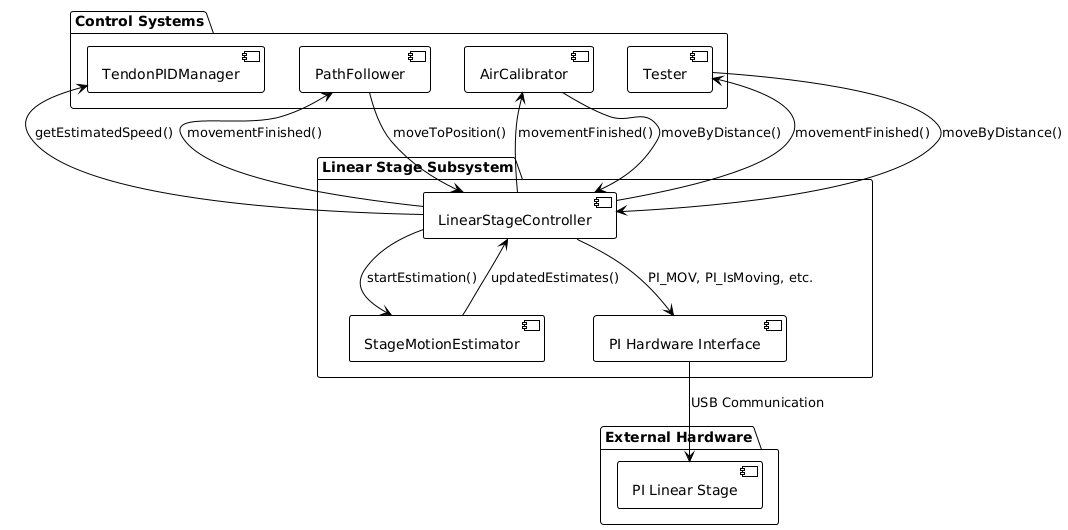
\includegraphics[width=\linewidth]{images/linearstage/architecture.png}
    \caption{Caption}
    \label{fig:enter-label}
\end{figure}

Two new classes were written to integrate this linear stage into the system software: \texttt{LinearStageController} and \texttt{StageMotionEstimator}. The \texttt{LinearStageController} is responsible for low-level communication with the linear stage hardware using the Physik Instrumente (PI) GCS2 API. It handles connection management, servo enable/disable commands, movement to absolute or relative positions, referencing, and safety checks for position limits and servo state. Timers are used to periodically check whether movement or referencing operations are complete, allowing the controller to emit signals when movement finishes or when feedback estimation should start or stop.
\newline \newline
Methods were also written for querying the current state of the system, such as position, speed, and servo status, and the class integrates with Qt’s signal-slot mechanism to communicate with other parts of the application. All interaction with the hardware is guarded by connection and safety checks to prevent invalid operations, and the use of QTimers ensures that blocking calls are avoided, keeping the GUI responsive. This modular and robust design makes the class easy and safe to  reuse and extend in future control experiments involving the linear stage.


\todo{figures of the new linearstage code}
\todo{picture of the linearstage}



\paragraph*{Implementing a motion estimator for the linear stage}
Although the GCS2 API for the linear stage offers some data transmission functionality, it lack the capability to continuously and reliably transmit real-time speed data at the necessary rate for feedforward control. Several lengthy and throrough attempts were made at using the PI data recorder system to fetch position readings (speed readings are not available through the recorder system). However it proved to have extremely limited buffer size leading it to either be too slow or limited in throughput for real-time control. Timer triggered querying was also attempted but since the API requires acknowledgements and the querying is slow this also was not a feasible solution.

\begin{figure}
    \centering
    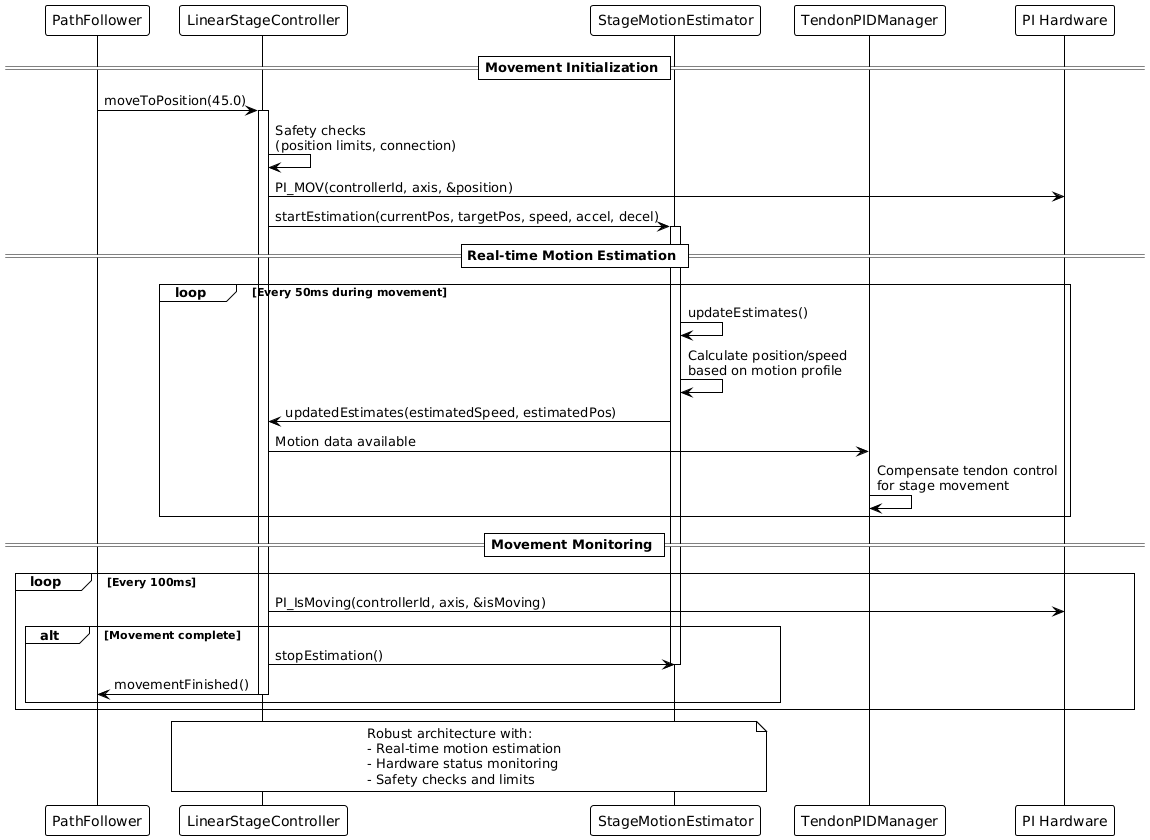
\includegraphics[width=\linewidth]{images/linearstage/movetopos_sequencediag.png}
    \caption{Caption}
    \label{fig:enter-label}
\end{figure}

The \texttt{StageMotionEstimator} class was therefore written to estimate the stage's speed and position. When a movement command is issued, this class is initialized with the start and target positions, as well as the target speed, acceleration and deceleration parameters. All parameters that are known and chosen by the user. It then calculates whether the motion will follow a trtapezoidal or triangular speed profile and starts a \texttt{QTimer} to periodically compute the current estimated speed and position. This allows for the access of real-time speed estimates for the feedforward, even though the stage hardware itself is incapable of supplying this information.
\todo{sequnce diagram for motion estimator}


\paragraph*{Linear stage speed ramping}
Because of the limitations of using a speed controller the dynamics of the system had to be slowed down like mentioned earlier. The motion profile of the linear stage was therefore adjusted to have much slower acceleration and deceleration than its default values \todo{put in acceleration values}. This is done since the speed of the linear stage is used as a feedforward for tension control, so ensuring that there are no quick jumps in linear stage speed will also ensure that there are not large jumps in motor setpoint speed thereby insuring that the inner speed loop has time to reach its setpoints.


\subsubsection{Tendon tension feedback controller}
The main component of the tension control system is the closed-loop feedback controller, which was re-implemented to address the issues identified in the earlier setup. The controller operates based on real-time force measurements obtained from the four tendon force sensors. The goal is to minimize the error between the measured tendon tension andthe desired setpoint, which can either be statically set or dynamically adjusted based on control objectives. 
\newline \newline
Each tendon has its own instance of the controller, which calculates the motor velocity required to minimize the error between the measured tendon tension and the desired setpoint. Each controller runs at a fixed interval of \SI{5}{\milli \second}, synchronized across al four tendons. The modular designa llows runtime adjustment of control parameters for each tendon.

\paragraph*{Sensor calibration}
Before reliable tension control could be implemented, substantial time was spend calibrating the tendon force sensors. Initially, there wree large discrepancies in the sensors outputs, where some sensors were measuring tension values that were up to five times too low compared to actual values. These errors were traced to misconfigured and miscalibrated sensors. To address this the sensor settings were changed. Specifically all settings were manually set to default values, except for resolution which was set to high-resulotion mode with  \SI{0.5}{\milli\volt\per\volt}, and the sampling frequency which was increased to \SI{1}{\kilo\hertz}. Since the PI cotroller runs at a fixed interval of \SI{5}{\milli\second}, it ensures that the sensor sampling rate is several times faster than the control loop update rate. After this the setting of the sensors was calibrated by using calibration weights to validate the force sensor read outs.

Additionally, a new tare function was implemented in the refactored \texttt{sensor} class to simplify the process of zeroing the sensors. This function sets the output voltage to \SI{10}{\volt} for a short period, triggering the sensor to register a zero-load state, and then resets the voltage back to zero. \texttt{Calibrate} buttons were also implemented in the GUI for each sensor so that this function can easily be called. This improves repeatability and reduces calibration drift over time.

\paragraph*{Motor deadzone}
During testing it was observed that the brushless motors ha d a certain deadzone, where a range of input voltages produced no movement of the motor due to internal friction, electrical thresholds or controller nonlinearity. In the tension control system that requires fine corrections, such unadressed deadzone behavior may cause delays and thereby oscillations and instability.
\newline \newline 
To quantify the deadzone, a motor was given a static voltage commands, incrementally increasing in both directions. It was observed that motion only behan at around \SI{1.5}{\volt}, regardless of direction. As a result, small acutation outputs below this threshold had no effect.
\newline \newline
To address this, a fixed \SI{1.5}{\volt} offset was added to all non-zero control signals, ensuring that outputs always exceeded the activation threshold. This improved responsiveness and significantly reduced oscillations and steady-state error, particularly during fine tension corrections or stage movement.

\paragraph*{PI controller}
The main component of the feedback controller is the PI controller. A PI controller was chosen for this application because of the system dynamics. The interaction between the tendon and surrounding gelatin result in a relatively slow and heavily damped system, making derivative control largely unnecessary and potentially counterproductive, as it tends to amplify noise. Proportional and integral terms were therefore deemed sufficient to drive the error to zero over time while maintaining smooth control. 
\newline \newline
The proportional gain provides immediate correction in response to tension deviations, while the integral term accumulates error over time to eliminate steady-state offset. However to prevent accumulation of too much error anti-windup was implemented. The integral term is also reset under specific conditions: when the setpoint changes, or when the linear stage starts or stops moving. These event introduce abrupt shifts in thhe system, making previous integral contributions invalid. By resetting the integral in these cases, the controller avoids reacting to outdated errors and ensures smoother, more accurate tension regulation. 

Looking at the PI_GCS2_DLL.h header, all the PI functions are synchronous blocking calls with no built-in timeout mechanism.

\paragraph*{Pull and release gains}
Since the mechanical dynamics of the system are dependent on whether you are increasing tension (pulling) or decreasing tension (releasing), each PI controller was implemented with two separate sets of gains. One for pulling and one for releasing. When pulling the motor must overcome the resistance from the ribbon pushing against the gelating, in contrast, when releasing the gelatin pushes the ribbon back, assisted by internal tension, leading to faster and less resistive motion. Intuitively the gains for the release must therefore be lower than those for pulling and by seperating the gain parameters each control direction could be tuned to better match these asymmetric dynamics.

\paragraph*{Tendon tension setpoint ramping}
To prevent instability in the outer tension control loop, the tension setpoints for the feedback were ramped gradually avoiding abrupt changes that the inner speed loop could not handle in time, which would otherwise cause overshoot, oscillations and instability.

\subsection{Results}

\begin{figure} [H]
    \centering
    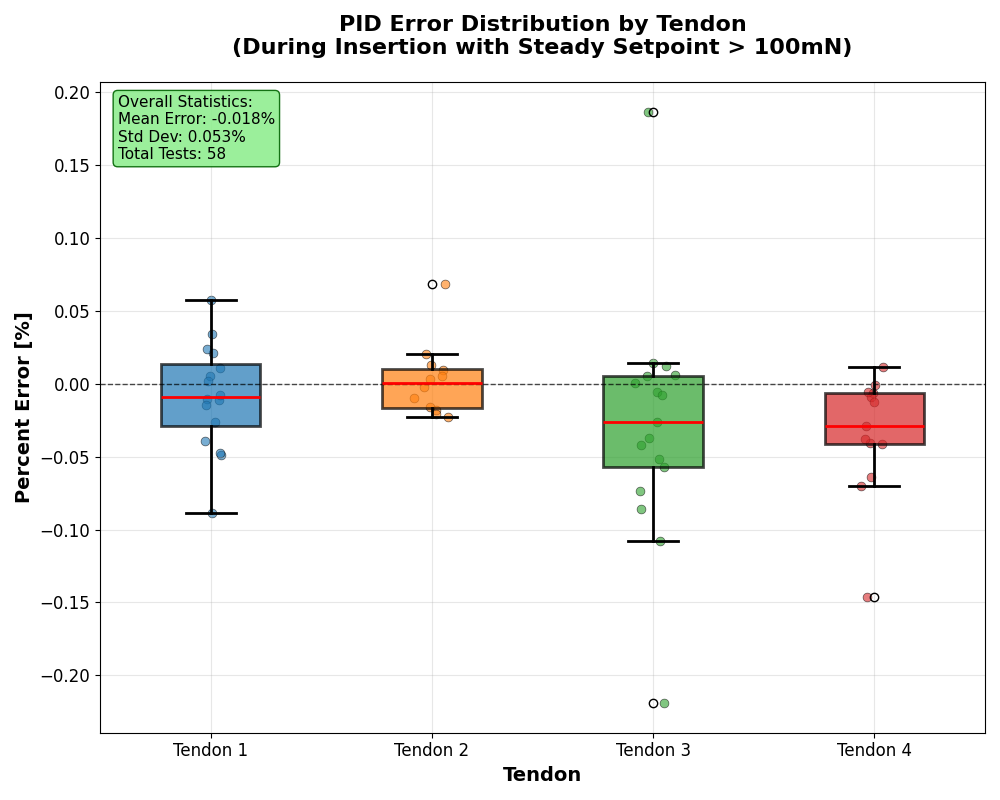
\includegraphics[width=0.9\linewidth]{images/PID performance/PIDErrorDistByTendon.png}
    \caption{Tension Control PID setpoint tracking error distribution by tendon during insertion with a steady setpoint above 100mN}
    \label{fig:PIDErrorDistByTendon}
\end{figure}

\begin{figure} [H]
    \centering
    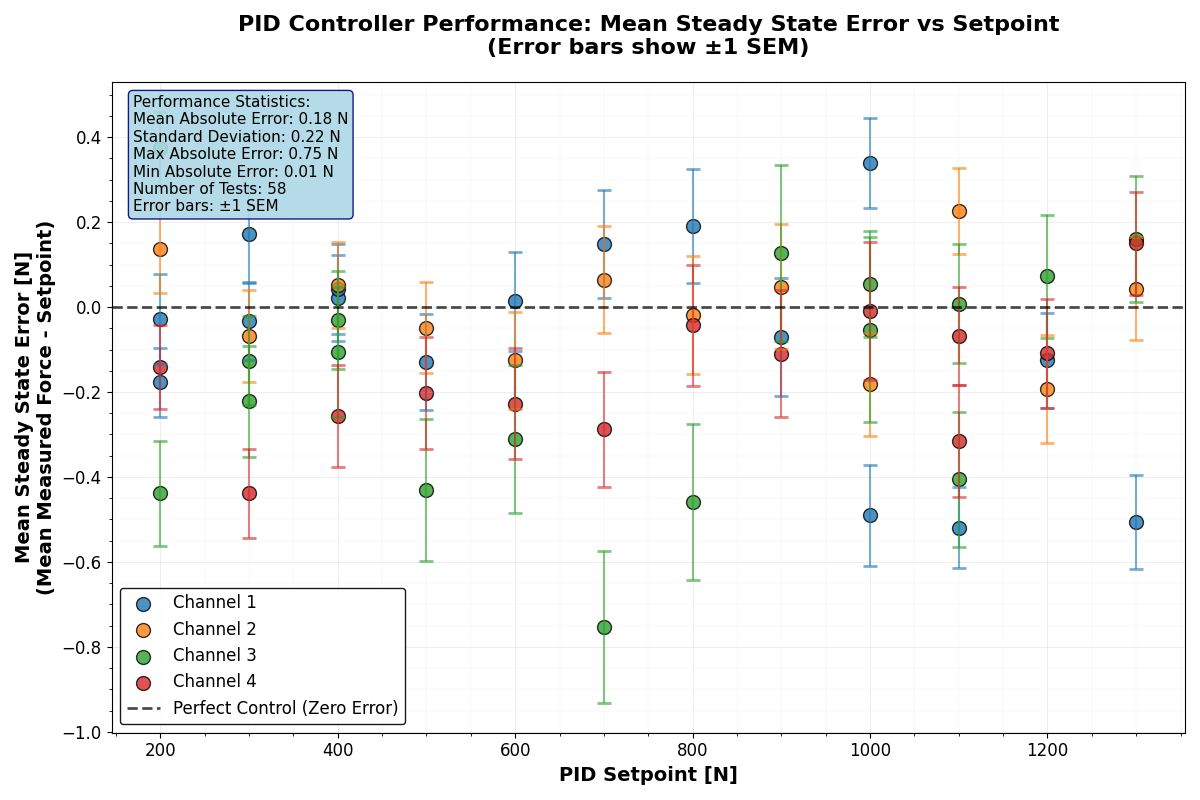
\includegraphics[width=0.9\linewidth]{images/PID performance/Figure_1.png}
    \caption{Mean Tension Control PID steady state error during insertion with steady setpoints above 100mN}
    \label{fig:steadtyStatePIDError}
\end{figure}

\begin{figure} [H]
    \centering
    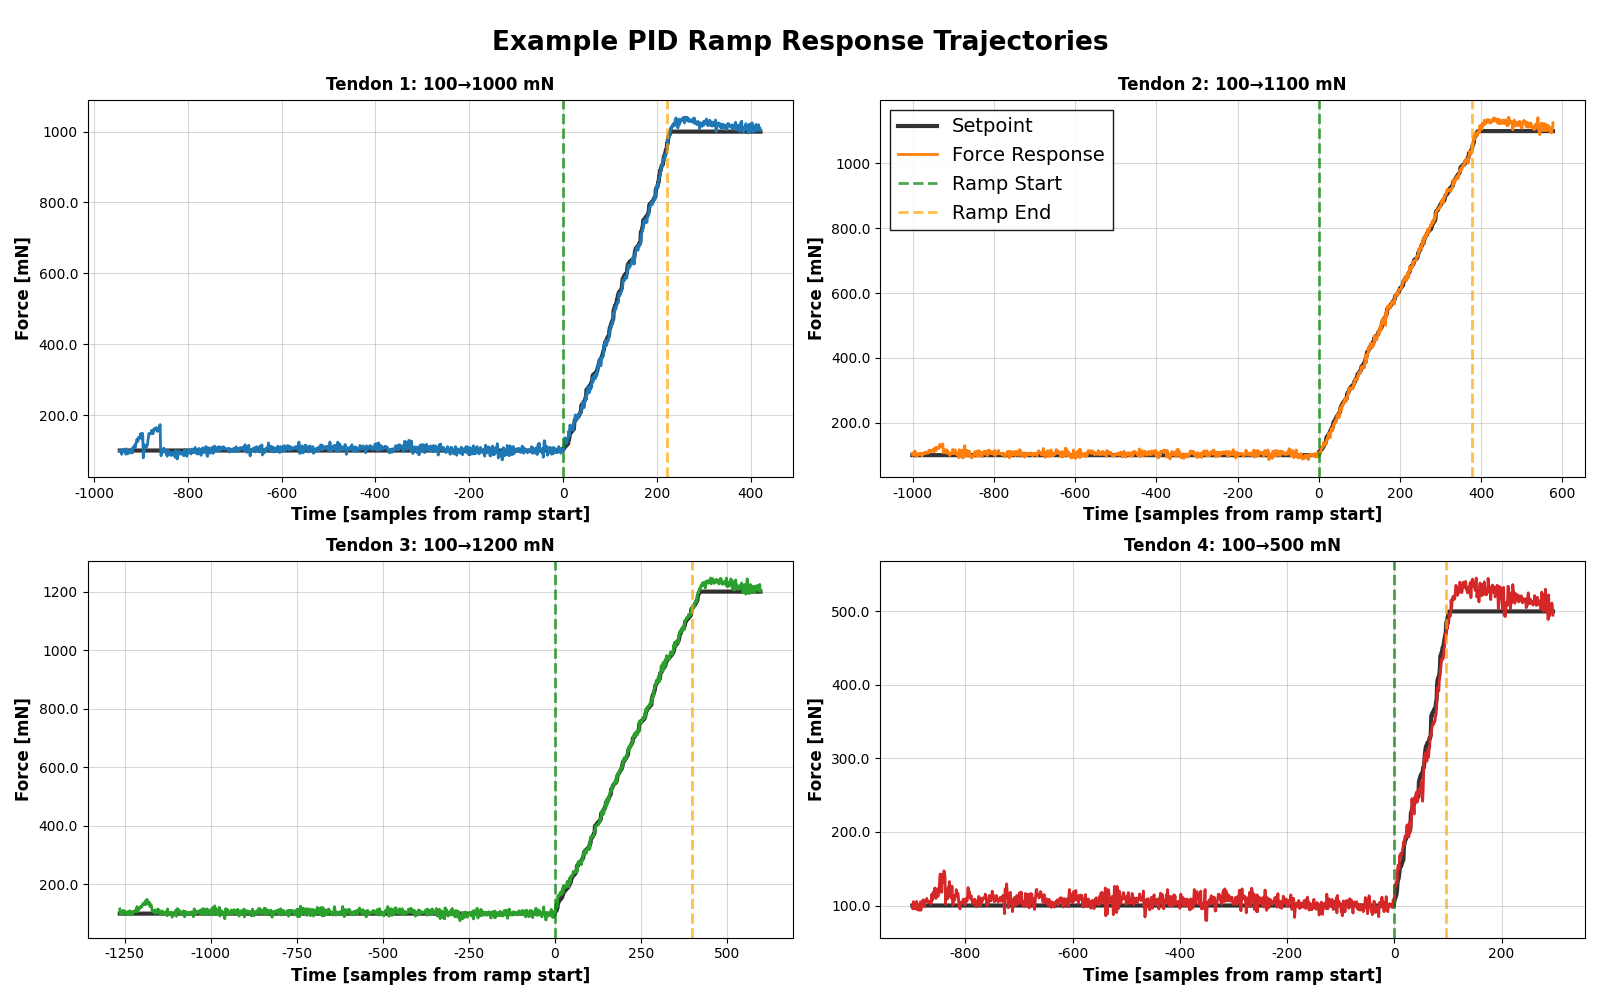
\includegraphics[width=\linewidth]{images/PID performance/rampExamples.png}
    \caption{Examples of measured tension during a ramping of setpoint while inserting the tendon}
    \label{fig:rampresponse}
\end{figure}

\subsection{Discussion}
